\section{Methodology}
\label{sec:methodology}

In this section, we introduce key steps of our works. We first detail how to sample points of fixed number for each sketch. Next, we explain our group scheme to choose a proper group size and guarantee the integrity of each group patterns. We then introduce our SketchPointNet architecture.

\subsection{Resample scenario}
\label{ssec:resample_scenario}

For each sketch, we sample it into a fixed number of points. The neighbor points inside a stroke have a fixed interval. We calculate each stroke length $\left\{ L_i| i = 1, ..., m \right\}$ from strokes $\left\{ T_i^{init}| i = 1, ..., m \right\}$. $m$ stands for stroke numbers. The total stroke length is $C$. Given the number of points $N$, we assign each stroke $B_i$ points $\left\{ B_i| i = 1, ..., m \right\}$ according to its corresponding stroke length $T_i$. Then we reample each stroke in $B_i$ points by using \$1 \cite{Wobbrock2007GesturesWL} resample scheme. The strokes after resampled are represented as $\left\{ T_i^{rsp}| i = 1, ..., m \right\}$. In Fig.~\ref{fig:resample}, the airplane and the tree are resample into different number of points.
\begin{algorithm}[h]
\label{alg:resample}
    \caption{Resample each sketch into N points}
    \KwIn{$\left\{ T_i^{init}| i = 1, ..., m \right\}$, resample number $N$}
    \KwOut{$\left\{ T_i^{rsp}| i = 1, ..., m \right\}$}
    $C = 0$\;
    \For{$ i = 1; i \le m $}
    {
        $L_i = |T_i^{init}|$\;
        $C = C + L_i$\;
    }

    \For{$ i = 1; i \le m $}
    {
        $B_i = \frac{L_i \times N}{C}$\;
        $T_i^{rsp} = single\_stroke\_resample(T_i^{init}, B_i)$\;
    }
    return $\left\{ T_i^{rsp}| i = 1, ..., m \right\}$\;
\end{algorithm}



\subsection{Group scheme}
\label{ssec:group_scheme}

After resampling sketches, we get each of them represented as N points $\left\{P_i| i = 1,..., N\right\}$. For a sketch, We resample a series of points $\left\{P_{1}, P_{1+t}, P_{1+2*t}, ..., P_{1+(S_g-1)*t}\right\}$ every $t$ points as group center from the N Points. Then we group points according to group center with radius $r$. After grouping the sketch, we get $N_{g} \times S_{g}$. $N_{g}$ is the number of the group center. $S_{g}$ is the points number of each group. In a similar way, we group the sketch for more times according to last grouping center.

The input group must have a fixed group size. Because tensorflow only supports static graph. But with a fixed group radius $r$, group size are very different from each other. After grouping the points, We get a series of groups. One of the groups contains $S_g$ group points $\left\{ Z_i| i = 1, ..., m \right\}$. If the group size is less than $S_{g}$, we pad the group center into the group till the group size is $S_{g}$. If the group size is greater than $S_{g}$, we delete group points every other points in the group till the group size is $S_{g}$. We develop an algorithm to guarantee the integrity of group patterns when deleting extra points.

\begin{algorithm}[h]
\label{alg:group}
    \caption{Delete extra points until group size is $S_g$}
    \KwIn{$\left\{ Z_i^{init}| i = 1, ..., m \right\}$, group size threshold $S_g$}
    \KwOut{$\left\{ Z_i| i = 1, ..., S_g \right\}$}
    $i = 2$\;
    $Z = Z^{init}$\;
    \While{$|Z| < S_g$}
    {
        \If{$i = |Z|+1$ or $i = |Z|+2$}
        {
            $i = 2$\;
        }
        del $Z_i$\;
        $i = i+1$\;
    }
    return $\left\{ Z_i| i = 1, ..., S_g \right\}$\;
\end{algorithm}

\begin{figure}
    \center
    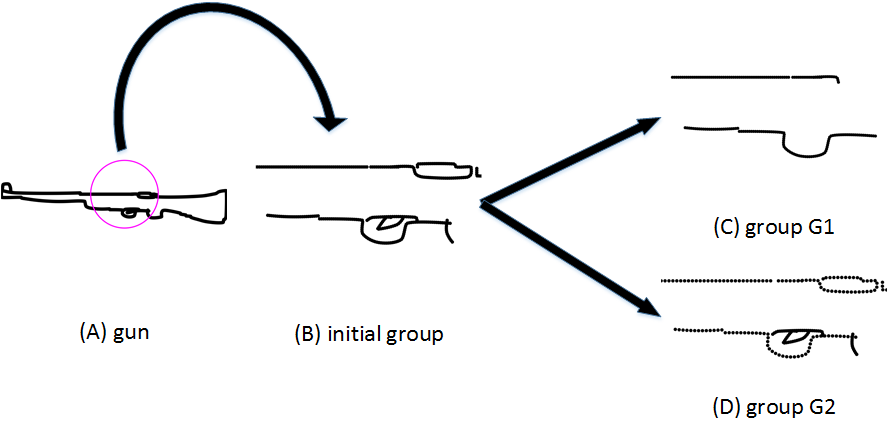
\includegraphics[width=3in]{images/group.png}
    \fcaption{Comparison of different group scheme. Group G2 contains more details than group G1.}
    \label{fig:group}
\end{figure}

All N points in a sketch are chronological. Grouping do not undermine the order of time series. The points in a group are still arranged in chronological order. In Fig.~\ref{fig:group} (B), we directly delete the last extra points to ensure that a group contains $S_g$ points. There are great loss of the pattern.  Algorithm ~\ref{alg:group} makes sure of the existence of the whole pattern(see Fig.~\ref{fig:group} (C)).

\subsection{SketchPointNet}
\label{ssec:sketch_point_net}

SketchPointNet architecture are borrowed from PointNet++ architecture. Each sketch is represented as 1024 points. We resample 512 points as group center every other points and group the points around the group center with a fixed radius. After the first time of grouping, we get 512 groups. Each group contains 20 points. We get group features after each of 512 groups pass through the micro PointNet.

With the group centers and its corresponding group features after first time of grouping, we group the points for the second time in a similar way. The group radius is larger than the first time with the need of a large receptive field. After two times of grouping, SketchPointNet can capture patterns of different receptive field.

\begin{figure}
    \center
    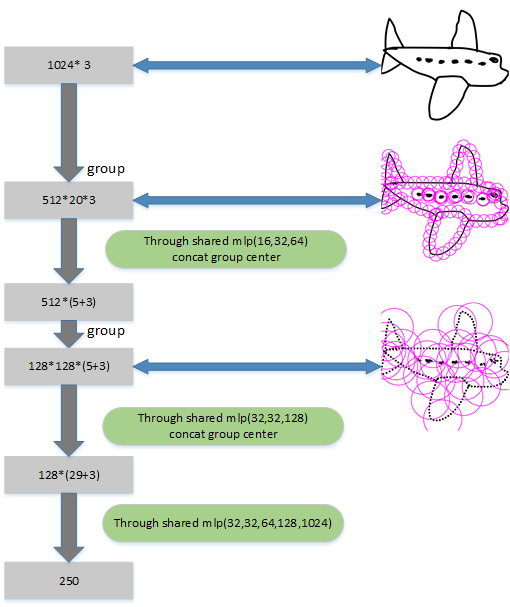
\includegraphics[width=3in]{images/sketchpointnet.png}
    \fcaption{SketchPointNet architecture.}
    \label{fig:sketchpointnet}
\end{figure}
